\let\negmedspace\undefined
\let\negthickspace\undefined
\documentclass[journal]{IEEEtran}
\usepackage[a5paper, margin=10mm, onecolumn]{geometry}
\usepackage{tfrupee}

\setlength{\headheight}{1cm}
\setlength{\headsep}{0mm}

\usepackage{gvv-book}
\usepackage{comment}
\usepackage{gvv}
\usepackage{cite}
\usepackage{amsmath,amssymb,amsfonts,amsthm}
\usepackage{algorithmic}
\usepackage{graphicx}
\usepackage{textcomp}
\usepackage{xcolor}
\usepackage{listings}
\usepackage{enumitem}
\usepackage{mathtools}
\usepackage{gensymb}
\usepackage[breaklinks=true]{hyperref}
\usepackage{tkz-euclide}
\usepackage{circuitikz}

\tikzstyle{block} = [rectangle, draw, fill=blue!20, 
    text width=4em, text centered, rounded corners, minimum height=3em]
\tikzstyle{sum} = [draw, fill=blue!10, circle, minimum size=1cm, node distance=1.5cm]
\tikzstyle{input} = [coordinate]
\tikzstyle{output} = [coordinate]

\begin{document}

\bibliographystyle{IEEEtran}
\vspace{3cm}

\title{12.755}
\author{EE25BTECH11013 - Bhargav}
\maketitle
{\let\newpage\relax\maketitle}

\renewcommand{\thefigure}{\theenumi}
\renewcommand{\thetable}{\theenumi}
\setlength{\intextsep}{10pt}

\numberwithin{equation}{enumi}
\numberwithin{figure}{enumi}
\renewcommand{\thetable}{\theenumi}

\textbf{Question}: \\
Which one of the following vectors is an eigenvector corresponding to the eigenvalue $\lambda = 1$ for the matrix 
\begin{align}
\vec{A} = \myvec{1 & 1 & 0 \\  1 & -1 & 0 \\ 1 & -1 & 1}
\end{align}
is

\solution \\

The eigenvalue of the the the matrix $\vec{A}$ can be found out by (where $\lambda=1$ is the eigenvalue, $\vec{x}$ is the eigenvector, $\vec{I}$ is the identity matrix)

\begin{align}
\vec{A}\vec{x} = \lambda \vec{x} \implies \vec{A}\vec{x} = \vec{x}
\end{align}
\begin{align}
\brak{\vec{A}-\vec{I}}\vec{x} = \vec{0}
\end{align}
\begin{align}
\implies \myvec{0 & 1 & 0 \\ 1 & -2 & 0 \\ 1 & -1 & 0}\vec{x} = \vec{0}
\end{align}


This can be solved by representing it as an augmented matrix and using row elimination
\begin{align}
\augvec{3}{1}{
0 & 1 & 0 & 0 \\
1 & -2 & 0 & 0 \\
1 & -1 & 0 & 0
}
\xleftrightarrow{R_1 \leftrightarrow R_2}
\augvec{3}{1}{
1 & -2 & 0 & 0 \\
0 & 1 & 0 & 0 \\
1 & -1 & 0 & 0
}
\xleftrightarrow{R_3 \leftarrow R_3 - R_1}
\end{align}
\begin{align}
\augvec{3}{1}{
1 & -2 & 0 & 0 \\
0 & 1 & 0 & 0 \\
0 & 1 & 0 & 0
}
\xleftrightarrow{R_3 \leftarrow R_3 - R_2}
\augvec{3}{1}{
1 & -2 & 0 & 0 \\
0 & 1 & 0 & 0 \\
0 & 0 & 0 & 0
}
\end{align}

Thus $\vec{x} = t\myvec{0 \\ 0 \\ 1}$ where $t \in \mathbf{R}$ \\
So, the eigenvector of $\vec{A}$ is $\myvec{0 \\ 0 \\ 1}$ \\ \\ \\

This can be further verified by the intersection of planes
\begin{align}
x - 2y = 0
\end{align}
\begin{align}
y = 0
\end{align}


The intersection of the 2 planes is $x=y=0$
    \begin{figure}[H]
        \centering
        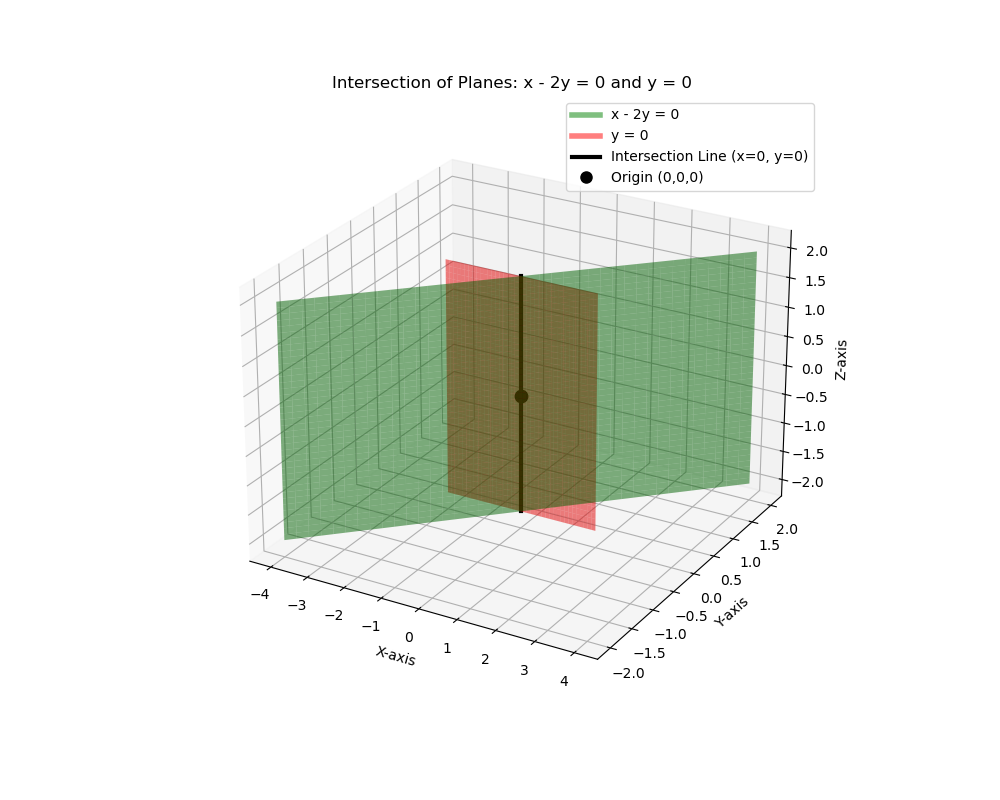
\includegraphics[height=0.5\textheight, keepaspectratio]{figs/Figure_1.png}
        \label{figure_1}
    \end{figure}
\end{document}
